\documentclass{article}

\usepackage{times}
\usepackage{geometry}
\geometry{a4paper,left=0.6cm,right=0.7cm,top=1.5cm,bottom=1cm,columnsep=0.8cm}

\usepackage{fontawesome}          % icônes de base seulement
\usepackage[hidelinks]{hyperref}
\usepackage{multicol}
\usepackage{tikz}
\usepackage{hyphsubst}
\usepackage{moresize}
\usepackage{hyphenat}
\usepackage{tabularx}
\usepackage{xcolor}
\usepackage{enumitem}
\usetikzlibrary{calc, positioning}
\newcolumntype{Y}{>{\RaggedRight\arraybackslash}X}

% icônes manquantes -> puce
\makeatletter
\@for\sym:=faBrain,faMicrochip,faHandshakeO,faTools,faNetworkWired,%
             faDatabase,faServer,faGit,faUsers,faComments,faCalendar,faGroup\do{%
  \@ifundefined{\sym}{\expandafter\newcommand\csname\sym\endcsname{\textbullet}}{}}
\makeatother

% couleurs
\definecolor{maincolor}{HTML}{f0fafc}
\definecolor{seccolor}{HTML}{ffffff}
\definecolor{gray}{HTML}{8c94a9}
\definecolor{sidetext}{HTML}{59cee5}

% bande latérale bleue
\usepackage{eso-pic}
\AddToShipoutPictureBG{%
  \begin{tikzpicture}[remember picture,overlay]
    \fill[maincolor] (current page.north west) rectangle
                     ([xshift=0.3\paperwidth] current page.south west);
  \end{tikzpicture}%
}

% listes
\setlist[itemize]{itemsep=-2pt,topsep=0pt,leftmargin=1.08cm}
\renewcommand{\labelitemi}{\textcolor{sidetext}{\footnotesize$\bullet$}}

\setlength{\parindent}{0pt}
\usepackage{paracol}
\columnratio{0.3}

\begin{document}
\pagestyle{empty}

\begin{paracol}{2}
% ────────────────────────────────────────
% Colonne gauche
% ────────────────────────────────────────
\color{sidetext}
\vspace*{-0.5cm}

\noindent
\begin{minipage}{\linewidth}
  \centering
  \begin{tikzpicture}
    \clip (0,0) circle (1.5cm) node[anchor=center]
      {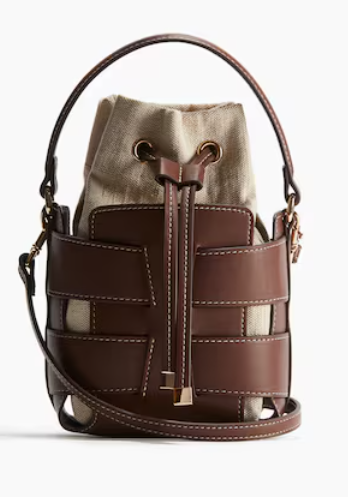
\includegraphics[width=3cm]{f22efc1d0eac4f378eca26230fb6a545.png}};
  \end{tikzpicture}

  \vspace{3mm}
  {\color{black}\LARGE \textbf{Pape Saliou Fall}}

  \vspace{1mm}
  {\large Ingénieur Data Scientist \& Développeur IA}

  \vspace{3mm}
  {\color{gray}\rule{\linewidth}{0.4pt}} \\
\end{minipage}

% ── Coordonnées
\begin{tabular}{@{}c l}
  \faPhone &
  \begin{tabular}[t]{@{}l@{}}
    {\color{gray}Téléphone} \\ 0753481453
  \end{tabular} \\
  \\
  \faLinkedin &
  \begin{tabular}[t]{@{}l@{}}
    {\color{gray}LinkedIn} \\
    \href{https://www.linkedin.com/in/pape-saliou-fall-43154a211/}{}
  \end{tabular} \\
  \\
  \faMapMarker &
  \begin{tabular}[t]{@{}l@{}}
    {\color{gray}Adresse} \\ 95300 Pontoise \\ 
  \end{tabular} \\
  \\
  \faEnvelope &
  \begin{tabular}[t]{@{}l@{}}
    {\color{gray}Email} \\
    \href{mailto:papesalioufall2@gmail.com}{papesalioufall2@gmail.com}
  \end{tabular} \\
\end{tabular}

\vspace{2mm}
{\color{gray}\rule{\linewidth}{0.4pt}} \\

% ── Langues --------------------------------------------------------
{\color{black}{Langues}}

\vspace{2mm}
\begin{itemize}[leftmargin=*]
\item Français - \textcolor{gray}{Maternel}
\item Anglais - \textcolor{gray}{B2}\end{itemize}          % ← le placeholder va contenir \begin{itemize}…\end{itemize}

{\color{gray}\rule{\linewidth}{0.4pt}} \\

% ── Compétences ----------------------------------------------------
\vspace{2mm}
{\color{black}{Compétences Clés}}

\vspace{2mm}
\begin{itemize}[leftmargin=*]
\item Python
\item SQL
\item TensorFlow
\item PowerBI
\item Git
\item Flask
\item NLP\end{itemize}              % ← idem, une vraie liste
\vspace{2mm}
{\color{gray}\rule{\linewidth}{0.4pt}} \\

% ── Centres d'intérêt
\vspace{2mm}
{\color{black}{Centres d’intérêt}}

\vspace{2mm}
\begin{itemize}[leftmargin=*]
\item Football
\item Natation
\item Lecture
\item Musique
\end{itemize}     % ← simple itemize ou tabular

\vfill
~

% ────────────────────────────────────────
\switchcolumn
% Colonne droite
% ────────────────────────────────────────
\color{black}

% ── Profil
\textcolor{black}{\Large \textbf{Profil Professionnel}} \\[2pt]
Ingénieur Data Scientist polyvalent, je combine une expertise en analyse de données, modélisation statistique et développement d’applications IA. Habitué à piloter des projets complets, je transforme des volumes d’informations complexes en solutions prédictives et opérationnelles. Autonome et proactif, j’apprécie le travail d’équipe pour relever des défis ambitieux et créer de la valeur. Je souhaite aujourd’hui évoluer dans un environnement innovant où mes compétences techniques et mon esprit d’initiative seront pleinement mobilisés. \\[8pt]

% ── Expérience
\textcolor{black}{\Large \textbf{Expérience Professionnelle}} \\[2pt]

\colorbox{maincolor}{%
  \begin{minipage}{\linewidth}
    \textbf{Data Scientist \& Développeur IA} \\ Prepaya \\ 01/2024 - Présent
    \begin{itemize}
      \item Conçu et développé une plateforme IA en Python et JavaScript, déployée sur Heroku pour un usage interne. \item Implémenté des modèles de Machine Learning et Deep Learning avec Scikit-learn, TensorFlow et Keras pour analyses prédictives. \item Réalisé des analyses de données et études de séries chronologiques afin de générer des insights opérationnels. \item Créé des API Flask connectées à OpenAI pour intégrer les services IA aux applications métiers. \item Supervisé le versionnement et la livraison continue via Git et GitHub.
    \end{itemize}
  \end{minipage}}

\vspace{3mm}


\colorbox{maincolor}{%
  \begin{minipage}{\linewidth}
    \textbf{Apprenti Risk Analyst \& Data Scientist} \\ AXA XL (Groupe AXA) \\ 12/2022 - 12/2023
    \begin{itemize}
      \item Automatisé la collecte des données financières du département avec Python et VBA. \item Développé des tableaux de bord Power BI pour la facturation, facilitant la prise de décision des équipes finance et management. \item Conçu une application analytique prédictive pour estimer la probabilité de survenance des sinistres. \item Écrit des requêtes sur SQL Server afin de consolider et fiabiliser les jeux de données sinistres. \item Maintenu le code et les rapports sous Visual Studio et Node.js, améliorant la maintenabilité des outils.
    \end{itemize}
  \end{minipage}}

\vspace{3mm}


\colorbox{maincolor}{%
  \begin{minipage}{\linewidth}
    \textbf{Apprenti Data Scientist} \\ Prepaya \\ 09/2021 - 08/2022
    \begin{itemize}
      \item Appliqué des techniques de Deep Learning en NLP pour générer automatiquement des formulaires clients. \item Réalisé des analyses de sentiments sur les retours clients pour évaluer la satisfaction. \item Développé des scripts de collecte de données avec BeautifulSoup et Selenium. \item Implémenté et testé des modèles BERT, T5 et TopicRank sous PyTorch pour extraire les informations clés.
    \end{itemize}
  \end{minipage}}   % ← blocs \colorbox{maincolor}{\begin{minipage}…}

\vspace{8mm}

% ── Formation
\textcolor{black}{\Large \textbf{Formation}} \\[2pt]

    \begin{tabularx}{\linewidth}{@{}c X@{}}
    \textcolor{sidetext}{\faGraduationCap} &
    \textbf{Master 2 Data Science} \\
    & Sorbonne Université \\
    & \begin{itemize}[leftmargin=*]
  \item Analyse de données avancée et séries chronologiques. \item Conception de modèles de Machine Learning, Deep Learning et apprentissage statistique. \item Gestion de bases de données, calcul parallèle et modèles de structure latente.
\end{itemize} \\
    & \textit{09/2021 - 03/2022}
    \end{tabularx}
           % ← lignes tabular par diplôme

\end{paracol}
\end{document}

